\documentclass[10pt,journal,a4paper]{IEEEtran}

\usepackage{amsmath,amssymb}
\usepackage{amsthm}
\usepackage{stmaryrd}
\usepackage{array}
\usepackage{booktabs}
\usepackage{enumitem}
\usepackage{microtype}
\usepackage{tikz}
\usepackage{tikz-cd}
\usepackage{cite}
\usepackage[hidelinks]{hyperref}

\hypersetup{
  pdfauthor={Ruiyi Zhang},
  pdftitle={A Categorical Semantics for PDE Energy Estimates: Proof Composition, Feature Lifting, and Analytic Transport},
  pdfsubject={Categorical semantics for PDE energy-estimate practice},
  pdfkeywords={PDE energy estimate, categorical semantics, proof graph, GS-monoidal category, abstract interpretation, proof lifting, analytic transport}
}

\usetikzlibrary{arrows.meta,positioning}
\setlist[enumerate]{leftmargin=1.8em,itemsep=0.2em,topsep=0.35em}
\setlength{\emergencystretch}{1.5em}

\newtheorem{theorem}{Theorem}[section]
\newtheorem{proposition}[theorem]{Proposition}
\theoremstyle{definition}
\newtheorem{definition}[theorem]{Definition}

\title{A Categorical Semantics for PDE Energy Estimates:\\
Proof Composition, Feature Lifting, and Analytic Transport}
\author{Ruiyi Zhang}

\begin{document}

\maketitle

\begin{abstract}
We give a categorical semantics for the operations used in PDE energy estimates. Fully specified estimates generate a proof category whose morphisms are rule-labeled term graphs; composition records successive inequalities, parallel morphisms record alternative arguments, and fan-out records reuse of an intermediate estimate. A semantic functor interprets this syntax by predicates on admissible PDE objects. Forgetting analytic data defines a feature functor. We prove that a local lifting condition on primitive rules is equivalent to lifting every finite abstract proof graph with prescribed concrete inputs. At the set level this condition yields the backward-completeness equation of abstract interpretation, while at the model level it identifies abstract truth models with feature-saturated concrete models. Global parameter compatibility is encoded by a constraint set on rule labels, and a feasible subfiber records realizations that satisfy the declared closure budget. Finally, budget-preserving analytic transports compose and send feasible proof certificates to feasible proof certificates.
\end{abstract}

\begin{IEEEkeywords}
PDE energy estimate, categorical semantics, proof graph, GS-monoidal category, abstract interpretation, proof lifting, analytic transport.
\end{IEEEkeywords}

\section{Introduction}

Let $E$ be a nonnegative energy and let $D=(D_1,\ldots,D_d)$ be nonnegative dissipation terms. An energy argument often reaches
\[
  \frac{1}{2}E'(t)+\lambda\mathbin{\cdot}D(t)
  \leq\sum_{\nu=1}^m N_\nu(t),
  \qquad 0<t<\mathcal T,
\]
where $\lambda\in(0,\infty)^d$. The analyst estimates the nonlinear terms by H\"older, Sobolev, interpolation, commutator, trace, Hardy, or problem-specific inequalities and then chooses Young parameters so that the total load returned to each dissipation component is smaller than the available budget.

The argument has a compositional structure. An estimate can be used as an input to another estimate, one intermediate estimate can feed several later steps, and different derivations can have the same conclusion. Exponent bookkeeping may describe a plausible proof plan even when no concrete choice of domain, boundary condition, regularity, parameter range, or uniform constant realizes the plan. A sequence of locally admissible parameter choices may still fail the final joint absorption test. A method can be moved to another PDE only after the transported premises, remainders, constants, and dissipation budget have been checked.

Table~\ref{tab:dictionary} is the organizing dictionary of the paper. The categorical objects are not introduced as analogies after the analysis has been completed; they are intended to encode the operations from which the analysis is assembled.

\begin{table*}[!t]
\centering
\small
\renewcommand{\arraystretch}{1.13}
\caption{A categorical dictionary for PDE energy-estimate practice.}
\label{tab:dictionary}
\begin{tabular}{>{\raggedright\arraybackslash}p{0.39\textwidth}
                >{\raggedright\arraybackslash}p{0.51\textwidth}}
\toprule
PDE analysis practice & Categorical representation \\
\midrule
A fully specified estimate & A generating object; a finite word is a context of available estimates \\
Using several estimates to derive another & A primitive multi-input box \\
Using inequalities successively & Composition \\
Carrying out independent estimates & Monoidal product \\
Reusing one intermediate estimate & Fan-out of a wire \\
Two different estimation routes & Parallel morphisms \\
Naming a calculation as a lemma & A generator identified with an existing composite \\
Shortening the displayed calculation & A shorter factorization in a chosen presentation, not a categorical invariant \\
Keeping only exponents or derivative orders & A feature functor \\
A plausible feature proof with no analytic realization & An abstract morphism with empty lifting fiber \\
Choosing Young or interpolation parameters & A point in a constrained lifting fiber \\
Locally valid choices that do not close & A nonempty lifting fiber with empty feasible subfiber \\
Moving a method to another PDE & An analytic transport functor \\
Comparing two transports coherently & A monoidal natural transformation, when its components and naturality are verified \\
\bottomrule
\end{tabular}
\end{table*}

Deductive systems have long been studied categorically \cite{Lambek1968,Meseguer1989}. Finite directed acyclic term graphs with visible sharing admit GS-monoidal presentations \cite{CorradiniGadducci1999,FritzLiang2023}. We use this structure because computing an estimate once and reusing it should not be identified with computing it twice. The resulting category is proof-relevant: its reachability preorder forgets parallel derivations and induces the usual rule-generated closure on judgments.

Abstract interpretation provides the order-theoretic language for sound abstraction and completeness \cite{CousotCousot1977,CousotCousot1979,GiacobazziRanzatoScozzari2000}. We apply it to the one-step transformer generated by the analytic rules and distinguish set-level backward completeness from lifting an individual proof graph. The local lifting condition is related to opfibrational ideas for multicategories \cite{Hermida2004}, but we require only existence of generator lifts and do not impose an opcartesian universal property.

Related computational work treats automatic symmetrization and energy estimates, symbolic conservation laws, or Lyapunov and dissipation certificates for specified PDE classes \cite{HagstromAppelo2007,Hereman2006,AhmadiValmorbidaPapachristodoulou2016,GahlawatValmorbida2020}. Category-theoretic work on differential equations has studied composition of physical models and computational representations \cite{PattersonBaasHosgoodFairbanks2023,MorrisEtAl2024}. Our object is the proof layer: analytic judgments, their derivations, partial abstractions of those derivations, global parameter compatibility, and transport of closing certificates. We make no priority claim for the general categorical constructions used here.

The contributions are as follows.
\begin{enumerate}[label=\emph{(\roman*)}]
  \item A sound analytic signature generates a GS-monoidal proof category and a semantic functor to predicates on admissible PDE objects. Rule closure and Galois polarity are obtained as proof-irrelevant shadows.
  \item A feature map induces a proof-graph functor. Local lifting of primitive boxes is equivalent to lifting every finite abstract proof graph with arbitrary concrete inputs. It also implies a backward-completeness equation for the one-step transformers and descent of feature-saturated truth models.
  \item One lifting fiber records concrete rule labels, while a separate constraint set records nonlocal parameter compatibility. Its feasible subfiber imposes the declared componentwise closure budget.
  \item Analytic transports are equipped with composable monotone budget maps. They preserve feasible certificates under explicit hypotheses, and natural transformations express coherent comparisons between two transports.
\end{enumerate}

Section~2 constructs the analytic proof category and its PDE semantics. Section~3 treats feature functors, proof lifting, abstract interpretation, and truth-model descent. Section~4 adds global constraints, feasible realizations, composable transports, and the scope of the formalism.

\section{Analytic proof categories and semantics}

\subsection{Notation and conventions}

All vector inequalities are componentwise. A finite word in a set $J$ is written $\mathbf x=(x_1,\ldots,x_k)$; the empty word is allowed. Concatenation is denoted by $\otimes$. If $q:J\to Q$, then $q\mathbf x=(q(x_1),\ldots,q(x_k))$. For $S\subseteq J$, the notation $\mathbf x\in S^{<\omega}$ means that every entry of $\mathbf x$ lies in $S$.

Fix an analytic context consisting of a spatial domain, a time interval, a class $\mathcal U$ of admissible PDE objects, boundary conditions, external PDE or approximation parameters, and a permitted class of constant dependences. External parameters remain formal coordinates. A constant in a judgment is a function of those coordinates in the permitted class; it is never made uniform by fixing an approximation parameter.

\subsection{Analytic signatures}

Let $J$ be a set of fully specified analytic judgments. The specification includes the quantities being estimated, domain and time interval, function spaces, boundary hypotheses, parameter ranges, and the declared dependence of constants. Let $R$ be a set of primitive analytic rule instances. An instance has a type
\[
  \rho:(x_1,\ldots,x_k)\longrightarrow y,
  \qquad k\geq1.
\]
A parameterized rule schema with admissible parameter set $P$ contributes one labeled instance to $R$ for every $\theta\in P$. Its type is given by a map
\[
  P\longrightarrow J^k\times J.
\]
Distinct parameter values remain distinct rule instances, even when their source and target judgments agree. An unparameterized rule uses a one-point parameter set.

An \emph{analytic signature} is a pair $\Sigma=(J,R)$. It is sound when, for every $u\in\mathcal U$ and every $\rho:(x_1,\ldots,x_k)\to y$ in $R$,
\[
  u\models x_1,\ldots,u\models x_k
  \quad\Longrightarrow\quad
  u\models y.
\]

\subsection{Proof graphs}

\begin{definition}\label{def:proof-category-v7}
The category $\mathsf{Der}(\Sigma)$ has finite words in $J$ as objects. A morphism
\[
  p:\mathbf x\longrightarrow\mathbf y
\]
is an isomorphism class of finite directed acyclic term graphs with ordered input interface $\mathbf x$ and ordered output interface $\mathbf y$. Wires are labeled by judgments. Each box is labeled by a rule $\rho:(z_1,\ldots,z_k)\to z$ and has ordered input ports with labels $z_1,\ldots,z_k$ and one output wire labeled $z$.

Every non-input wire has a unique producing box. A wire may feed several later box ports, may occur at several output ports, or may be unused after it is produced. Composition glues matching interfaces, tensor product is disjoint union, and identities are unbroken interface wires.
\end{definition}

The following graph displays one intermediate estimate $z$ used by two later rules.
\[
\resizebox{0.94\columnwidth}{!}{%
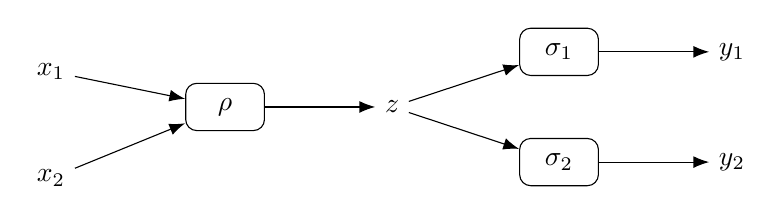
\begin{tikzpicture}[
  node distance=9mm and 14mm,
  box/.style={draw,rounded corners,minimum width=10mm,minimum height=6mm},
  every edge/.style={draw,-{Latex[length=2mm]}}
]
  \node (x1) {$x_1$};
  \node[below=of x1] (x2) {$x_2$};
  \node[box,right=of x1,yshift=-4.5mm] (rho) {$\rho$};
  \node[right=of rho] (z) {$z$};
  \node[box,right=of z,yshift=7mm] (s1) {$\sigma_1$};
  \node[box,right=of z,yshift=-7mm] (s2) {$\sigma_2$};
  \node[right=of s1] (y1) {$y_1$};
  \node[right=of s2] (y2) {$y_2$};
  \path (x1) edge (rho);
  \path (x2) edge (rho);
  \path (rho) edge (z);
  \path (z) edge (s1);
  \path (z) edge (s2);
  \path (s1) edge (y1);
  \path (s2) edge (y2);
\end{tikzpicture}
}
\]

The category in Definition~\ref{def:proof-category-v7} is the free GS-monoidal category on the typed rule signature. Copying and discarding are visible as fan-out and unused wires, but they are not natural with respect to analytic boxes. Thus the graph above is not identified with a graph containing two copies of $\rho$, and an unused analytic computation is not erased \cite{CorradiniGadducci1999,FritzLiang2023}.

\subsection{Analytic semantics}

Let $\mathsf{Pred}(\mathcal U)$ be the category whose objects are subsets of $\mathcal U$ and whose morphisms are inclusions. Its tensor product is intersection and its unit is $\mathcal U$. For $x\in J$, set
\[
  \llbracket x\rrbracket
  =
  \{u\in\mathcal U:u\models x\},
\]
and for a word $\mathbf x=(x_1,\ldots,x_k)$ set
\[
  \llbracket\mathbf x\rrbracket
  =
  \bigcap_{i=1}^k\llbracket x_i\rrbracket,
  \qquad
  \llbracket()\rrbracket=\mathcal U.
\]

\begin{proposition}\label{prop:analytic-semantics}
The signature $\Sigma$ is sound if and only if the assignment on judgments extends to a GS-monoidal functor
\[
  \llbracket-\rrbracket:
  \mathsf{Der}(\Sigma)
  \longrightarrow
  \mathsf{Pred}(\mathcal U).
\]
\end{proposition}

\begin{proof}
A primitive box $\rho:(x_1,\ldots,x_k)\to y$ has an image in $\mathsf{Pred}(\mathcal U)$ precisely when
\[
  \bigcap_{i=1}^k\llbracket x_i\rrbracket
  \subseteq
  \llbracket y\rrbracket,
\]
which is the soundness implication for $\rho$. If all primitive boxes are sound, the universal property of the free proof category gives the functor. Conversely, applying the functor to a primitive box gives the displayed inclusion.
\end{proof}

This functor is the analytic meaning of the proof syntax. It forgets parallel proofs because $\mathsf{Pred}(\mathcal U)$ is thin, but it retains the distinction between a syntactic proof and its validity for the declared PDE objects.

\subsection{Reachability and the Galois shadow}

For $S\subseteq J$, define
\[
  \operatorname{reach}_\Sigma(S)
  =
  \left\{
  y\in J:
  \begin{array}{l}
    \mathsf{Der}(\Sigma)(\mathbf x,(y))\neq\varnothing\\
    \text{for some }\mathbf x\in S^{<\omega}
  \end{array}
  \right\}.
\]
The existence of a morphism defines a preorder on context words. Restricting its source to finite words in $S$ and its target to singletons gives the closure above.

\begin{proposition}
The map $S\mapsto\operatorname{reach}_\Sigma(S)$ is the finitary closure generated by $R$. If $\Sigma$ is sound and $u\models s$ for every $s\in S$, then
\[
  y\in\operatorname{reach}_\Sigma(S)
  \quad\Longrightarrow\quad
  u\models y.
\]
\end{proposition}

\begin{proof}
A topological ordering of a proof graph gives a finite rule derivation. Conversely, a finite derivation is a proof tree and hence a term graph. The soundness conclusion follows either by induction along the graph or by Proposition~\ref{prop:analytic-semantics}.
\end{proof}

Let $\mathbf2$ be the ordered category $0<1$, with tensor product given by conjunction. A \emph{truth model} is a GS-monoidal functor
\[
  M:\mathsf{Der}(\Sigma)\longrightarrow\mathbf2.
\]
Truth models correspond to rule-stable subsets $Z\subseteq J$: if all premises of a rule lie in $Z$, then its conclusion lies in $Z$. For every $u\in\mathcal U$, the assignment
\[
  M_u(x)=1
  \quad\Longleftrightarrow\quad
  u\models x
\]
is a truth model when $\Sigma$ is sound. Not every truth model need arise from an admissible PDE object.

For $X\subseteq J$, let $\operatorname{Mod}(X)$ be the truth models assigning $1$ to every element of $X$. For a set $\mathcal M$ of truth models, let $\operatorname{Th}(\mathcal M)$ be the judgments assigned $1$ by every model in $\mathcal M$. Then
\[
  \mathcal M\subseteq\operatorname{Mod}(X)
  \quad\Longleftrightarrow\quad
  X\subseteq\operatorname{Th}(\mathcal M),
\]
and
\[
  \operatorname{reach}_\Sigma(X)
  =
  \operatorname{Th}(\operatorname{Mod}(X)).
\]
Thus $(\operatorname{Mod},\operatorname{Th})$ is the Galois polarity between judgments and syntactic obstructions. It is complete for reachability, not for the existence of an analytic counterexample.

\subsection{Derived rules}

Let $\mathcal C$ be a GS-monoidal category presented by the typed generators $R$ and a fixed set of relations, and let $p:\mathbf x\to(y)$ be represented by an old proof graph. Adjoin a generator $\ell:\mathbf x\to(y)$ and the relation $\ell=p$.

\begin{proposition}
Adding $\ell$ together with the relation $\ell=p$ gives a presentation of a category isomorphic to $\mathcal C$.
\end{proposition}

\begin{proof}
The functor sending $\ell$ to $p$ and fixing the old generators is inverse to the inclusion of the old presentation.
\end{proof}

This is a Tietze-type conservative extension \cite{HenryMimram2022}. It formalizes naming an existing calculation as a lemma and may shorten its displayed factorization, but no presentation-independent complexity is asserted. If $\ell$ is adjoined without the equation, it is a new parallel proof; reachability is still unchanged when the old proof $p$ exists. If no old proof with that type exists, adjoining a sound rule is a genuine deductive extension and may enlarge reachability.

\section{Feature functors, lifting, and abstraction}

\subsection{Feature signatures and lifting fibers}

Let $\overline\Sigma=(Q,\overline R)$ be a feature signature. A \emph{surjective feature map}
\[
  q:\Sigma\longrightarrow\overline\Sigma
\]
consists of surjections on judgments and primitive rules that preserve ordered premises and conclusions. It induces a GS-monoidal functor
\[
  q_*:\mathsf{Der}(\Sigma)
  \longrightarrow
  \mathsf{Der}(\overline\Sigma).
\]
The feature judgment may retain only a quantity type, derivative order, space-time exponents, and energy or dissipation degree. Domain, boundary, regularity, and constant information can remain in the concrete fiber.

Let $p:\mathbf a\to\mathbf b$ be an abstract proof graph, let $q\mathbf x=\mathbf a$, and let $A$ be a set of concrete output words satisfying $q\mathbf y=\mathbf b$ for every $\mathbf y\in A$. Define
\[
\begin{aligned}
  &\operatorname{Lift}_q(p;\mathbf x,A)\\
  &\quad=
  \bigl\{\widetilde p:\mathbf x\to\mathbf y\mid
  \mathbf y\in A,\ q_*(\widetilde p)=p\bigr\}.
\end{aligned}
\]
When $A$ is the entire concrete word fiber over $\mathbf b$, we write $\operatorname{Lift}_q(p;\mathbf x)$.

\begin{definition}\label{def:local-lifting-v7}
The feature map $q$ has the \emph{local rule-lifting property} if, for every abstract rule
\[
  \overline\rho:(a_1,\ldots,a_k)\longrightarrow c
\]
and every $x_i\in J$ satisfying $q(x_i)=a_i$, there is a concrete rule
\[
  \rho:(x_1,\ldots,x_k)\longrightarrow y
\]
such that $q(\rho)=\overline\rho$ and $q(y)=c$.
\end{definition}

\begin{theorem}\label{thm:lifting-v7}
For a surjective feature map $q:\Sigma\to\overline\Sigma$, the following are equivalent.
\begin{enumerate}[label=\emph{(\roman*)}]
  \item The map $q$ has the local rule-lifting property.
  \item For every finite abstract proof graph $p:\mathbf a\to\mathbf b$ and every concrete input word $\mathbf x$ with $q\mathbf x=\mathbf a$,
  \[
    \operatorname{Lift}_q(p;\mathbf x)\neq\varnothing.
  \]
\end{enumerate}
When these conditions hold, for every $S\subseteq J$,
\begin{equation}\label{eq:feature-reach-v7}
  q\bigl[\operatorname{reach}_\Sigma(S)\bigr]
  =
  \operatorname{reach}_{\overline\Sigma}\bigl(q[S]\bigr).
\end{equation}
\end{theorem}

\begin{proof}
Assume local lifting. Order the boxes of $p$ topologically and fix the concrete input labels. When a box is reached, all its incoming wires have concrete labels. Definition~\ref{def:local-lifting-v7} supplies a compatible concrete rule and an output in the required feature fiber. A shared wire receives one concrete label and keeps it at every later use. Iterating over the finite graph gives a lift.

Conversely, apply part \emph{(ii)} to a graph containing one abstract primitive box and arbitrary concrete representatives of its inputs.

The inclusion from left to right in \eqref{eq:feature-reach-v7} follows by applying $q_*$. For the reverse inclusion, choose representatives in $S$ for the finite abstract input word and lift the abstract proof graph.
\end{proof}

The theorem gives a generator-level existence condition. It does not provide chosen opcartesian lifts or their universal property, so we do not identify it with an opfibration of multicategories \cite{Hermida2004}. It is also stronger than equality of reachable feature sets: a different concrete proof can reach the same feature even when the specified abstract graph has no lift.

For a prescribed concrete target $\mathbf y$, lifting every abstract graph from $q\mathbf x$ to $q\mathbf y$ is exactly surjectivity of
\[
  \mathsf{Der}(\Sigma)(\mathbf x,\mathbf y)
  \longrightarrow
  \mathsf{Der}(\overline\Sigma)(q\mathbf x,q\mathbf y).
\]
This hom-wise property is stronger than Theorem~\ref{thm:lifting-v7}, which allows the concrete output to vary inside its feature fiber.

\subsection{Failure localization}

Let $\tau$ be an abstract proof tree with leaf features and abstract rule labels. Fix $S\subseteq J$. For each vertex $v$, define $L_v\subseteq J$ recursively. If $v$ is a leaf labeled by $a_v$, set
\[
  L_v=\{x\in S:q(x)=a_v\}.
\]
If $v$ has children $v_1,\ldots,v_k$ and rule label
\[
  \overline\rho_v:(a_1,\ldots,a_k)\longrightarrow c,
\]
let $L_v$ be the concrete conclusions $y$ of rules
\[
  \rho:(x_1,\ldots,x_k)\longrightarrow y
\]
with $x_i\in L_{v_i}$, $q(\rho)=\overline\rho_v$, and $q(y)=c$.

\begin{proposition}
The tree $\tau$ has a concrete lift with leaves in $S$ if and only if $L_{\mathrm{root}}\neq\varnothing$. If every leaf set is nonempty but the root set is empty, there is an internal vertex $v$ such that every child set is nonempty and $L_v=\varnothing$.
\end{proposition}

\begin{proof}
The first statement is induction from the leaves. For the second, start at an empty root and move to an empty child whenever one exists. Finiteness and nonempty leaf sets force the process to stop at an empty internal vertex whose children have nonempty sets.
\end{proof}

The empty set at $v$ can record a boundary mismatch, excluded endpoint, regularity loss, incompatible constant policy, or another local type failure. For a DAG, the same wire constrains several later boxes, so exact realization is a finite constraint system on the entire graph; a minimal obstruction can be a subgraph rather than one vertex.

\subsection{The Cousot--Cousot shadow}

Define the concrete one-step transformer
\[
\begin{aligned}
  F_\Sigma(S)=S\cup\bigl\{y\in J:{}&
  \rho:\mathbf x\to y,\ \rho\in R,\\
  &\mathbf x\in S^{<\omega}\bigr\}.
\end{aligned}
\]
and define $F_{\overline\Sigma}$ analogously. For $X\subseteq J$ and $W\subseteq Q$, the object map of $q$ gives
\[
  \alpha(X)=q[X],
  \qquad
  \gamma(W)=q^{-1}[W],
\]
with
\[
  \alpha(X)\subseteq W
  \quad\Longleftrightarrow\quad
  X\subseteq\gamma(W).
\]
Surjectivity of $q$ makes this a Galois insertion.

\begin{proposition}
For every $S\subseteq J$,
\[
  \alpha F_\Sigma(S)
  \subseteq
  F_{\overline\Sigma}\alpha(S).
\]
If $q$ has the local rule-lifting property, then
\begin{equation}\label{eq:backward-complete-v7}
  \alpha F_\Sigma
  =
  F_{\overline\Sigma}\alpha.
\end{equation}
\end{proposition}

\begin{proof}
A concrete rule step relabels to an abstract rule step, which proves the inclusion. Conversely, suppose an abstract rule is applied to features in $\alpha(S)$. Choose a representative in $S$ for each premise. Local lifting supplies a concrete rule with those premises and an output in the required feature fiber. This proves the reverse inclusion.
\end{proof}

Equation~\eqref{eq:backward-complete-v7} expresses backward completeness for the chosen abstract transformer \cite{GiacobazziRanzatoScozzari2000}. Iterating it gives equation \eqref{eq:feature-reach-v7}. The converse need not hold: set equality can be witnessed by a concrete proof graph different from the abstract graph under consideration.

\subsection{Descent of truth models}

Precomposition with $q_*$ sends an abstract truth model to a concrete truth model. Call a concrete truth model \emph{feature-saturated} if
\[
  q(x)=q(x')
  \quad\Longrightarrow\quad
  M(x)=M(x').
\]

\begin{proposition}
If $q$ has the local rule-lifting property, precomposition with $q_*$ is a bijection between truth models of $\overline\Sigma$ and feature-saturated truth models of $\Sigma$.
\end{proposition}

\begin{proof}
The pullback of an abstract model is feature-saturated. Conversely, let $M$ be a feature-saturated concrete model and define $\overline M(a)=M(x)$ for any $x$ with $q(x)=a$. This is well defined. If
\[
  \overline\rho:(a_1,\ldots,a_k)\longrightarrow c
\]
has all premises true in $\overline M$, choose concrete representatives $x_i$. Local lifting supplies
\[
  \rho:(x_1,\ldots,x_k)\longrightarrow y
\]
over $\overline\rho$. Stability of $M$ gives $M(y)=1$, hence $\overline M(c)=1$. Thus $\overline M$ is a truth model. Surjectivity on judgments makes pullback injective.
\end{proof}

This proposition connects the feature functor to the Galois polarity: abstract obstructions are exactly the concrete obstructions that are insensitive to information forgotten by $q$.

\section{Constrained realizations and analytic transport}

\subsection{Global constraint data}

A concrete lift already records the parameter value of every primitive rule instance. Nonlocal requirements need additional data. Let $p$ be an abstract proof graph and label its boxes by $\overline\rho_v$. A \emph{constraint set} for $p$ is a subset
\[
  \Gamma_p
  \subseteq
  \prod_v q^{-1}(\overline\rho_v),
\]
where the product is indexed by the boxes of $p$. It can impose equality of parameters used at different boxes, common endpoint choices, uniformity restrictions, or any other declared compatibility condition on the concrete rule labels.

For $A$ in the output word fiber of $p$, define
\[
\begin{aligned}
  &\operatorname{Lift}_q(p;\mathbf x,A\mid\Gamma_p)\\
  &\quad=
  \bigl\{\widetilde p\in\operatorname{Lift}_q(p;\mathbf x,A):\\
  &\qquad (\rho_v)_v\in\Gamma_p\bigr\},
\end{aligned}
\]
where $\rho_v$ is the concrete rule label of the box $v$ in $\widetilde p$.

Theorem~\ref{thm:lifting-v7} concerns local type compatibility and does not imply that this constrained fiber is nonempty. Shared parameters turn realization into a global finite constraint system even when every box has an individual lift. This is the formal distinction between an exponent-level proof plan, a concrete proof graph, and a globally compatible realization.

\subsection{Feasible realizations}

Fix a dissipation budget $\lambda\in(0,\infty)^d$. Suppose each constrained lift $\widetilde p$ has a load
\[
  b_p(\widetilde p)\in[0,\infty)^d
\]
and a fully specified remainder. In the componentwise direct-absorption setting, the load records how much of each dissipation coefficient is consumed by the nonlinear estimates. Call the remainder admissible when it belongs to the declared remainder and constant classes. Define
\[
\begin{aligned}
  &\operatorname{Feas}_q(p;\mathbf x,A\mid\Gamma_p)\\
  &\quad=
  \bigl\{\widetilde p\in
  \operatorname{Lift}_q(p;\mathbf x,A\mid\Gamma_p):\\
  &\qquad b_p(\widetilde p)<\lambda,\\
  &\qquad \text{the remainder is admissible}\bigr\}.
\end{aligned}
\]

Thus $\operatorname{Lift}_q$ records concrete realizability, $\Gamma_p$ records global compatibility, and $\operatorname{Feas}_q$ records passage of the declared closure test. The condition $b_p(\widetilde p)<\lambda$ is part of the analytic specification rather than a separate result of the categorical formalism. A different closure mechanism can be represented by replacing the load space and its feasible region.

\subsection{Composable analytic transports}

For this subsection, a \emph{budgeted analytic system} consists of a feature map together with declared input and output classes, constraint sets for abstract proof graphs, admissible remainder and constant classes, a load map on each constrained lifting fiber, and a dissipation budget. These data are part of the system; none is inferred from the feature signature alone.

Let $q:\Sigma\to\overline\Sigma$ and $q':\Sigma'\to\overline\Sigma'$ be feature maps. A signature map sends judgments and primitive rules to judgments and primitive rules while preserving ordered sources and targets. An analytic transport consists of signature maps $T$ and $\overline T$ forming a commuting square
\[
\begin{tikzcd}[column sep=large]
  \Sigma \arrow[r,"T"] \arrow[d,"q"']
    & \Sigma' \arrow[d,"q'"] \\
  \overline\Sigma \arrow[r,"\overline T"']
    & \overline\Sigma' .
\end{tikzcd}
\]
They induce a commuting square of proof-graph functors. The transport maps rule-instance parameters, declared constant dependences, constraint sets, and acceptable output families. For fixed compatible proof data, write $p'=\overline T_*p$ and assume
\[
\begin{aligned}
  T_*:\quad&
  \operatorname{Lift}_q(p;\mathbf x,A\mid\Gamma_p)\\
  &\longrightarrow
  \operatorname{Lift}_{q'}
  (p';T\mathbf x,A'\mid\Gamma'_{p'}).
\end{aligned}
\]

Let the source and target budgets be $\lambda\in(0,\infty)^d$ and $\lambda'\in(0,\infty)^{d'}$. A \emph{budget map} for $T$ is a monotone function
\[
  \beta_T:[0,\infty)^d\longrightarrow[0,\infty)^{d'}
\]
such that
\[
  b_{p'}(T_*\widetilde p)
  \leq
  \beta_T\bigl(b_p(\widetilde p)\bigr)
\]
for every constrained lift and
\[
  b<\lambda
  \quad\Longrightarrow\quad
  \beta_T(b)<\lambda'.
\]
Affine budget bounds are special cases. We use $\beta_T$ as the primary datum because monotone maps compose without additional linear structure.

\begin{theorem}
Assume that $T$ sends verified source inputs to verified target inputs, acceptable source outputs to acceptable target outputs, source constraints to target constraints, and admissible remainders and constant dependences to their target classes. If $T$ has a budget map $\beta_T$, then
\[
\begin{aligned}
  T_*:\quad&
  \operatorname{Feas}_q(p;\mathbf x,A\mid\Gamma_p)\\
  &\longrightarrow
  \operatorname{Feas}_{q'}(p';T\mathbf x,A'\mid\Gamma'_{p'}).
\end{aligned}
\]
\end{theorem}

\begin{proof}
For a feasible lift $\widetilde p$, one has $b_p(\widetilde p)<\lambda$. The budget-map condition gives
\[
  b_{p'}(T_*\widetilde p)
  \leq
  \beta_T\bigl(b_p(\widetilde p)\bigr)
  <\lambda'.
\]
The remaining assumptions give the target input, output, constraint, remainder, and constant conditions.
\end{proof}

\begin{proposition}
Identity analytic transports have identity budget maps. If $T_1$ and $T_2$ are composable analytic transports with budget maps $\beta_{T_1}$ and $\beta_{T_2}$, then $T_2T_1$ is an analytic transport with budget map
\[
  \beta_{T_2T_1}
  =
  \beta_{T_2}\circ\beta_{T_1}.
\]
Thus budgeted analytic systems and their compatible transports form a category, and feasible certificates move covariantly.
\end{proposition}

\begin{proof}
The identity statement is immediate. For composition, apply the two load inequalities successively and use monotonicity of $\beta_{T_2}$. The two feasible-cone inclusions compose, as do the maps of proof graphs, constraints, remainders, and constants.
\end{proof}

Truth-valued obstructions move contravariantly: if
\[
  M':\mathsf{Der}(\Sigma')\longrightarrow\mathbf2
\]
is a truth model, then $M'\circ T_*$ is a source truth model. In particular, a target model that contains $T(S)$ and excludes $T(y)$ proves that $y\notin\operatorname{reach}_\Sigma(S)$.

\subsection{Comparing transports}

Let $(T_0,\overline T_0)$ and $(T_1,\overline T_1)$ be two analytic transports between the same budgeted systems. A \emph{categorical comparison} consists of monoidal natural transformations
\[
  \eta:T_{0*}\Longrightarrow T_{1*},
  \qquad
  \overline\eta:\overline T_{0*}\Longrightarrow\overline T_{1*},
\]
compatible with the feature functors in the sense that
\[
  q'_*\eta_{\mathbf x}
  =
  \overline\eta_{q\mathbf x}
\]
for every context word $\mathbf x$. The concrete transformation assigns a proof graph
\[
  \eta_{\mathbf x}:T_0\mathbf x\longrightarrow T_1\mathbf x
\]
such that, for every $p:\mathbf x\to\mathbf y$,
\[
  \eta_{\mathbf y}\circ T_{0*}(p)
  =
  T_{1*}(p)\circ\eta_{\mathbf x}.
\]
Its components also satisfy $\eta_{\mathbf x\otimes\mathbf y}=\eta_{\mathbf x}\otimes\eta_{\mathbf y}$ and $\eta_{()}=\operatorname{id}_{()}$, with analogous identities for $\overline\eta$. This is the categorical meaning of a coherent comparison between two methods at both the analytic and feature levels. Preservation of constraint sets and admissible remainders requires further comparison data. A numerical assertion that one method has a smaller closure load requires an inequality between their budget maps; naturality alone does not provide it.

\subsection{Scope}

The framework begins after the analytic judgments, primitive inequalities, admissible PDE objects, and constant policies have been specified. It does not prove a Sobolev, trace, commutator, or boundary estimate, and it does not show that a useful feature map satisfies local lifting. Shared parameter constraints, target premises, and transport hypotheses must be verified for each application.

Truth-valued obstructions are syntactic non-reachability certificates and need not be analytic counterexamples. The load cone $[0,\infty)^d$ represents componentwise budgets; coupled coercivity or matrix-valued dissipation requires a different ordered budget space. We have not imposed a universal quantitative enrichment because constants can add, multiply, take powers, or enter nonlinear remainder functions under composition. Convex feature relaxation, automated search, and model-specific realizability are left for later work.

\subsection*{Version information}

This document is the v1 public release. Release timestamp: \texttt{2026-07-20T01:43:43+08:00}.

\subsection*{Declaration on generative AI}

OpenAI's ChatGPT and Codex were used during brainstorming, structural editing, and language revision. They were not treated as sources for mathematical or bibliographic claims. Responsibility for the mathematical statements and citations remains with the author.

\begin{thebibliography}{99}

\bibitem{AhmadiValmorbidaPapachristodoulou2016}
M.~Ahmadi, G.~Valmorbida, and A.~Papachristodoulou,
\emph{Dissipation inequalities for the analysis of a class of PDEs},
Automatica \textbf{66} (2016), 163--171,
\href{https://doi.org/10.1016/j.automatica.2015.12.010}{doi:10.1016/j.automatica.2015.12.010}.

\bibitem{CorradiniGadducci1999}
A.~Corradini and F.~Gadducci,
\emph{An algebraic presentation of term graphs, via GS-monoidal categories},
Applied Categorical Structures \textbf{7} (1999), no.~4, 299--331,
\href{https://doi.org/10.1023/A:1008647417502}{doi:10.1023/A:1008647417502}.

\bibitem{CousotCousot1977}
P.~Cousot and R.~Cousot,
\emph{Abstract interpretation: a unified lattice model for static analysis of programs by construction or approximation of fixpoints},
in \emph{Conference Record of the Fourth Annual ACM SIGPLAN--SIGACT Symposium on Principles of Programming Languages}, 1977, pp.~238--252,
\href{https://doi.org/10.1145/512950.512973}{doi:10.1145/512950.512973}.

\bibitem{CousotCousot1979}
P.~Cousot and R.~Cousot,
\emph{Systematic design of program analysis frameworks},
in \emph{Conference Record of the Sixth Annual ACM SIGPLAN--SIGACT Symposium on Principles of Programming Languages}, 1979, pp.~269--282,
\href{https://doi.org/10.1145/567752.567778}{doi:10.1145/567752.567778}.

\bibitem{FritzLiang2023}
T.~Fritz and W.~Liang,
\emph{Free GS-monoidal categories and free Markov categories},
Applied Categorical Structures \textbf{31} (2023), article~21,
\href{https://doi.org/10.1007/s10485-023-09717-0}{doi:10.1007/s10485-023-09717-0}.

\bibitem{GahlawatValmorbida2020}
A.~Gahlawat and G.~Valmorbida,
\emph{Stability analysis of linear partial differential equations with generalized energy functions},
IEEE Transactions on Automatic Control \textbf{65} (2020), no.~5, 1924--1939,
\href{https://doi.org/10.1109/TAC.2019.2927711}{doi:10.1109/TAC.2019.2927711}.

\bibitem{GiacobazziRanzatoScozzari2000}
R.~Giacobazzi, F.~Ranzato, and F.~Scozzari,
\emph{Making abstract interpretations complete},
Journal of the ACM \textbf{47} (2000), no.~2, 361--416,
\href{https://doi.org/10.1145/333979.333989}{doi:10.1145/333979.333989}.

\bibitem{HagstromAppelo2007}
T.~Hagstrom and D.~Appel\"o,
\emph{Automatic symmetrization and energy estimates using local operators for partial differential equations},
Communications in Partial Differential Equations \textbf{32} (2007), no.~7, 1129--1145,
\href{https://doi.org/10.1080/03605300600854258}{doi:10.1080/03605300600854258}.

\bibitem{HenryMimram2022}
S.~Henry and S.~Mimram,
\emph{Tietze equivalences as weak equivalences},
Applied Categorical Structures \textbf{30} (2022), no.~3, 453--483,
\href{https://doi.org/10.1007/s10485-021-09662-w}{doi:10.1007/s10485-021-09662-w}.

\bibitem{Hereman2006}
W.~Hereman,
\emph{Symbolic computation of conservation laws of nonlinear partial differential equations in multi-dimensions},
International Journal of Quantum Chemistry \textbf{106} (2006), no.~1, 278--299,
\href{https://doi.org/10.1002/qua.20727}{doi:10.1002/qua.20727}.

\bibitem{Hermida2004}
C.~Hermida,
\emph{Fibrations for abstract multicategories},
in \emph{Galois Theory, Hopf Algebras, and Semiabelian Categories},
Fields Institute Communications, vol.~43, American Mathematical Society, 2004, pp.~281--293,
\href{https://doi.org/10.1090/fic/043/11}{doi:10.1090/fic/043/11}.

\bibitem{Lambek1968}
J.~Lambek,
\emph{Deductive systems and categories I: syntactic calculus and residuated categories},
Mathematical Systems Theory \textbf{2} (1968), no.~4, 287--318,
\href{https://doi.org/10.1007/BF01703261}{doi:10.1007/BF01703261}.

\newpage
\bibitem{Meseguer1989}
J.~Meseguer,
\emph{General logics},
in \emph{Logic Colloquium '87}, Studies in Logic and the Foundations of Mathematics, vol.~129, North-Holland, 1989, pp.~275--329,
\href{https://doi.org/10.1016/S0049-237X(08)70132-0}{doi:10.1016/S0049-237X(08)70132-0}.

\bibitem{MorrisEtAl2024}
L.~Morris, A.~Baas, J.~Arias, M.~Gatlin, E.~Patterson, and J.~P. Fairbanks,
\emph{Decapodes: a diagrammatic tool for representing, composing, and computing spatialized partial differential equations},
Journal of Computational Science \textbf{81} (2024), article~102345,
\href{https://doi.org/10.1016/j.jocs.2024.102345}{doi:10.1016/j.jocs.2024.102345}.

\bibitem{PattersonBaasHosgoodFairbanks2023}
E.~Patterson, A.~Baas, T.~Hosgood, and J.~Fairbanks,
\emph{A diagrammatic view of differential equations in physics},
Mathematics in Engineering \textbf{5} (2023), no.~2, 1--59,
\href{https://doi.org/10.3934/mine.2023036}{doi:10.3934/mine.2023036}.

\end{thebibliography}

\end{document}
2026-07-20T01:43:34:z
